\begin{problem}{Bridges in Liyue}{standard input}{standard output}{1 second}{256 megabytes}

In Genshin Impact, the protagonist Traveler excels at using teleport waypoints for fast travel. Specifically, the Traveler can teleport from any location to the designated teleport waypoint.

In the Huaguang Stone Forest of Liyue, there are several extremely high peaks that are nearly impossible to climb, connected by wooden bridges. Among these peaks, only one has a teleport waypoint.

\begin{center}
  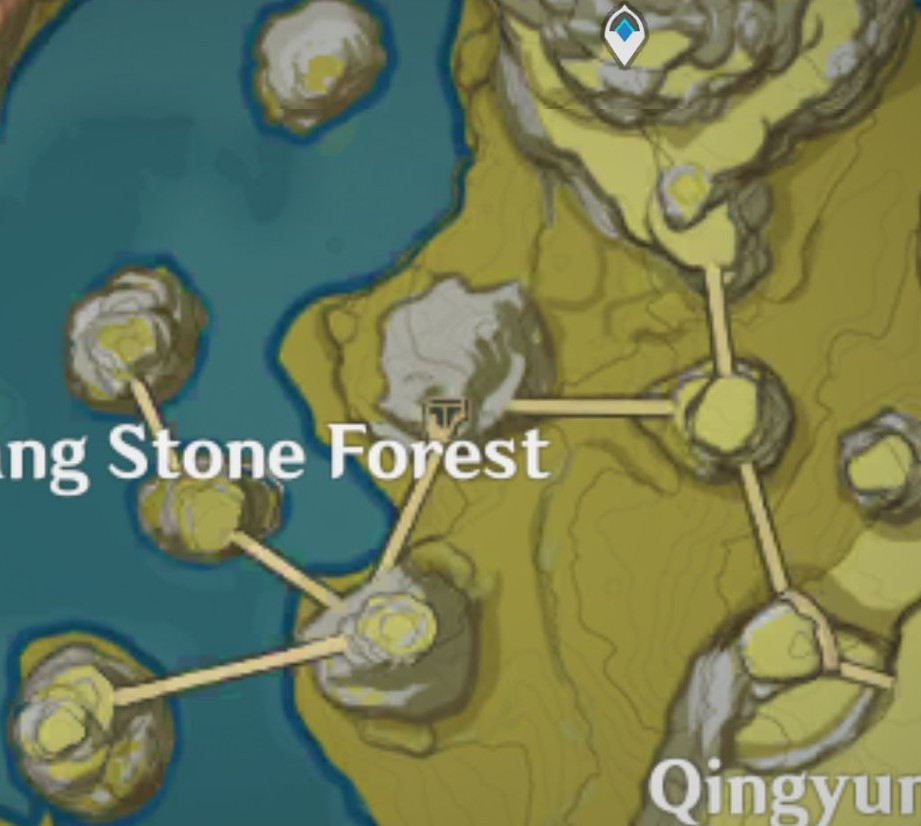
\includegraphics[scale=0.8]{path.jpg} \\
  \small{Huaguang Stone Forest}
\end{center}

Recently, the Traveler received a commission to inspect these bridges. In order to minimize the inspection time, the Traveler hopes to find a path that \textbf{starts from the teleport waypoint}, passes through each bridge exactly once, and can \textbf{end at any peak}.

Your task is to determine whether the path the Traveler is looking for exists.

\InputFile
The first line consists of two integers, $n$ and $m$, representing the number of peaks and the number of bridges. The peak with the teleport waypoint is designated as peak $1$. ($3 \le n \le 200$,$2 \le m \le \dfrac{n(n - 1)}{2}$)

The following $m$ lines each contain two integers, $u$ and $v$, indicating a bridge connecting peaks $u$ and $v$. ($1 \le u < v \le n$)

It is guaranteed that any peak can be reached from the teleport waypoint, and there is no pair of bridges connecting the same pair of peaks.

\OutputFile
If the path exists, output ``YES''; otherwise, output ``NO''. The checker is case-insensitive.


\Examples

\begin{example}
\exmpfile{example.01}{example.01.a}%
\exmpfile{example.02}{example.02.a}%
\exmpfile{example.03}{example.03.a}%
\end{example}

\end{problem}

